\chapter{驾驭项目成本}
\section{项目成本管理概述}
成本管理存在的问题
\begin{enumerate}
	\item 从小开始的教育就没有注意灌输成本的概念。
	\item 对IT项目的原始成本估算不准确。
	\item 项目组成员对成本估算和控制不相关。
	\item 项目组成员对成本的理解和把握不准确。
	\item 认为项目成本增长和失败将不可避免的。
\end{enumerate}
\subsection{项目成本与项目成本管理}
\subsubsection{项目成本的定义}
项目成本是指为完成项目目标而付出的费用和耗费的资源。
\par 项目成本包括项目决策和定义成本、项目获取成本、项目设计成本、项目实施成本等。项目实施成本是项目总成本的主要组成部分。
\par IT项目成本包括硬件成本、软件成本、项目集成成本、人力资源成本、场所成本、外包服务成本等。
\par 软件项目成本包括开发生产成本(分析设计成本、系统实施成本)和运行维护成本(专业培训成本、系统运行成本、维护改进成本和行政管理成本)等。
\subsubsection{成本管理的定义}
项目成本管理就是在整个项目的实施过程中,为确保项目在批准的预算条件下尽可能保质按期完成,而对所需的各个过程进行管理与控制。
\subsubsection{成本管理过程}
\begin{itemize}
	\item 成本估算:对完成项目所需成本的估计和计划,是项目计划中的一个重要的、关键的、敏感的部分。
	\item 成本预算:把估算的总成本分配到项目的各个工作细目,建立成本基准计划以衡量项目绩效。
	\item 成本控制:保证各项工作在各自的预算范围内进行。
\end{itemize}
\begin{figure}[!h]
	\centering
	
\includegraphics[width=0.8\textwidth]{image/6-1}
	\caption{项目成本管理过程图}
\end{figure}
\subsection{影响IT项目成本的因素}
影响成本的因素:质量、进度、范围。
\par 另外一些影响因素:系统规模类成本因素、数据库类成本因素、系统复杂性类的成本因素、软件开发类的成本因素、编写文档类的成本因素、环境与项目属性类的成本因素。
\subsection{成本管理的基本原理}
管理者最关心的是财务指标。
\begin{itemize}
	\item 利润 = 收入— 成本 
	\item 利润率 = 利润/收入
	\item 全生命期成本 = 开发成本 + 维护成本
	\item 现金流分析:对现金及现金等价物的流入与流出量的分析。
	\item 内部收益率:是使净现值等于零的折现率,它也被称为时间调整收益率。
	\item 有形成本/有形收益:能够以货币衡量的成本或收益。 
	\item 无形成本/无形收益:难用货币来衡量的成本或收益。
	\item 直接成本:能够以一种很经济的方式加以追踪的相关成本。
	\item 间接成本:不能以一种很经济的方式加以追踪的相关成本。
	\item 沉没成本:永远不可能再产生收益的成本。
	\item 学习曲线理论:当重复生产许多产品时,产品的单位成本随着数量的增多成规律性递减。 
\end{itemize}
\section{项目成本估算}
\subsection{成本估算的类型}
\begin{figure}[!h]
	\centering
	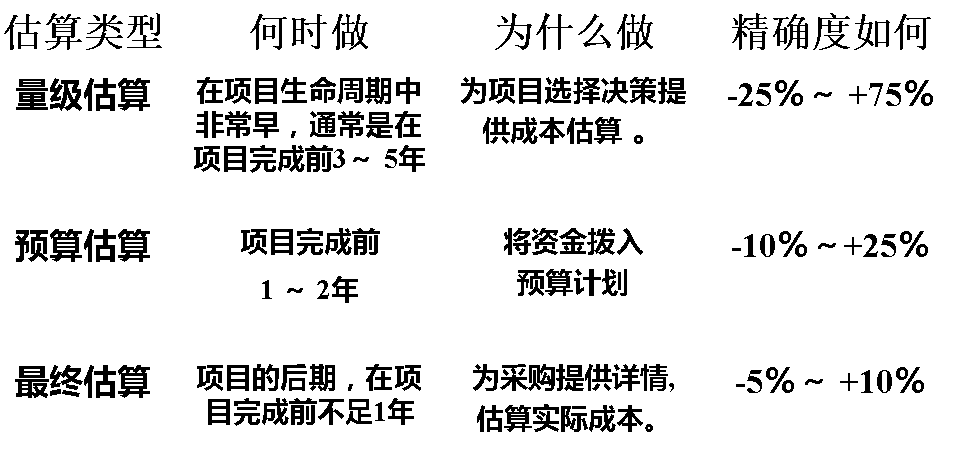
\includegraphics[width=0.8\textwidth]{image/6-2}
	\caption{项目成本估算类型}
\end{figure}
\subsection{成本估算的依据与输出}
主要依据:项目资源需求计划、项目范围说明书、项目进度计划、工作分解结构、
风险管理计划、相关历史资料和经验教训。
\par 主要成果:
\begin{itemize}
	\item 成本估算
	\item 估算的详细依据,包括采用的基本规则,估算所用的假设、基础资料、工具和技术。
	\item 成本管理计划,一份描述如何管理项目中成本变化的文件。
\end{itemize}
\subsection{项目成本估算方法}
\begin{itemize}
	\item 类比估算法:也叫专家判断法,是一种在成本估算精确程度要求不高的情况下使用的方法。它比照以前的、相似项目的实际成本作为目前项目成本估算的根据,来估算出当前项目的成本。
	\item 自上而下估算法:基于中上层管理人员的经验和判断、以及可以获得的关于以往类似项目的历史数据来进行项目成本估算的方法。
	\item 自下而上估算法:先估算单个工作项成本,然后从下往上汇总成整体项目成本。
	\item 参数模型估算法:在数学模型中应用项目特征参数来估算项目成本的方法。
\end{itemize}
\section{项目成本预算}
项目费用预算主要包括,直接人工费用、咨询服务费用、资源采购费用和不可预见费用等的预算。
\par 项目成本预算的主要依据包括项目成本估算、WBS和项目进度计划。
\par 成本预算过程的主要目标是制定一个成本基准计划以衡量项目绩效。
\subsection{成本预算的特征}
\begin{enumerate}
	\item 计划性:预算是另一种形式的项目计划。
	\item 约束性:预算是一种分配资源的计划,预算分配的结果可能并不能满足所涉及的管理人员的利益要求,而表现为一种约束,所涉及人员只能在这种约束的范围内行动。
	\item 控制性:项目预算是一种控制机制。预算可以作为一种比较标准而使用,一种度量资源实际使用量和计划量之间差异的基线标准。
\end{enumerate}
\subsection{成本预算的编制}
\begin{itemize}
	\item 确定项目的总预算:总预算确定的目的是为了将资金拨入预算计划,其精度提高到-10\%~25\%。
	\item 项目各项活动的预算:采用“自上而下”的方法,确定项目各项活动的预算。
	\item 项目各项活动预算投入的时间:根据项目的进度安排和项目的资源供应计划,确定各项活动预算投入的时间。
\end{itemize}
\subsection{成本基准计划}
项目成本基准计划是一个按时间分布的、用于测量和监控成本实施情况的预算,
是项目成本控制的基础,它为成本控制过程提供有效的依据。
\par 成本基准计划随时间的关系是一个S型曲线。
\subsection{不可预见费用分析}
不可预见费用是指为项目在实施过程中发生意外而准备的保证金,也就是在成本管理原理中提到的储备金.
\par 两种类型:
\begin{itemize}
	\item 显在的不可预见费用,通常在项目文件中明确标明。
	\item 潜在的不可预见费用,通常在项目文件中没有标明。对应成本管理原理中提到的应急储备金和管理储备金。
\end{itemize}
\section{项目成本控制}
有效的成本控制的关键在于及时分析成本的绩效,尽早发现成本无效和出现偏差的原因,以便在项目成本失控之前能够及时采取纠正措施。
\par 项目成本控制必须与项目的其他控制过程紧密结合,防止单纯的控制项目成本而出现项目范围、进度、质量等方面的问题。
\subsection{成本控制的内容}
\par 项目成本控制的主要内容:
\begin{enumerate}
	\item 监控实际成本与计划成本的偏差;
	\item 确认费用偏差都被记录;
	\item 避免不正确、不合适的或者无效的费用变更发生;
	\item 获取项目变更的各种信息,特别关注影响对成本变更的消息。
\end{enumerate}
\subsection{成本控制的依据}
\begin{itemize}
	\item 成本基准:成本基准是按时间分段的预算,用做度量和监控项目整体成本的基准。
	\item 绩效报告:绩效报告是提供实际工作中项目成本和资源绩效的信息。
	\item 请求变更:对项目的某些方面提出一些修改的要求。这些变更申请对成本的使用方向以及对成本的预算产生影响,可能增加成本,也可能减少成本。
	\item 成本管理计划:描述当项目实际成本和计划成本发生差异时如何进行管理,对整个成本控制过程进行有序的安排,可以实现对成本合理安排与使用。
\end{itemize}
\subsection{成本控制的方法}
\begin{enumerate}
	\item 成本变更控制系统:从请求变更,到批准请求变更,一直到最终变更项目成本预算的整个变更控制过程。
	\item 成本绩效测量法:帮助项目管理者及时分析项目成本状况,尽早发现项目成本差异,争取在情况变坏之前采取措施予以纠正。挣值分析法就是一种有效的分析方法,可用于进行项目成本偏差分析和控制。
	\item 附加计划法:通过新增或修订原有计划来对项目成本进行有效的控制。
	\item 计算机辅助法:借助相关的项目管理软件,跟踪项目的计划成本、实际成本和预测成本改变的影响。
\end{enumerate}
\subsection{挣值分析法}
挣值分析是一种项目绩效测量技术,它综合了范围、时间和成本数据。它是项目管理领域中有一个特有的、非常有效的成本控制工具。
\par 挣值法实际上是一种分析目标实施与目标期望之间差异的方法。故而它又被称为偏差分析法,通过测量和计算已完成的工作的预算费用和实际费用以及计划工作的预算费用得到计划实施的进度和费用的偏差,达到判断项目预算和进度计划执行情况的目的。
\par 挣值法的三个基本参数:
\begin{itemize}
	\item 计划工作量的预算成本(BCWS) :BCWS是指计划要求完成的工作量所需的预算工时/费用。 
	\subitem BCWS = 计划工作量 * 预算定额
	\item 已完成工作的实际成本(ACWP) :ACWP是指实际完成的工作量所消耗的工时/费用。
	\item 已完成工作量的预算成本(BCWP) :BCWP是指实际完成的工作量按预算定额计算的工时/费用。 
	\subitem BCWP =实际工作量 *预算定额
\end{itemize}
三者关系:
\begin{itemize}
	\item 已完成工作量的预算成本>已完成工作的实际成本,即BCWP>ACWP,效率高,反之效率低;
	\item 已完成工作量的预算成本>计划工作量的预算成本,即BCWP>BCWS,进度快,反之进度慢;
	\item 已完成工作的实际成本>计划工作量的预算成本,即ACWP>BCWS,投入超前,反之投入延后。
\end{itemize}

\begin{figure}[!h]
	\centering
	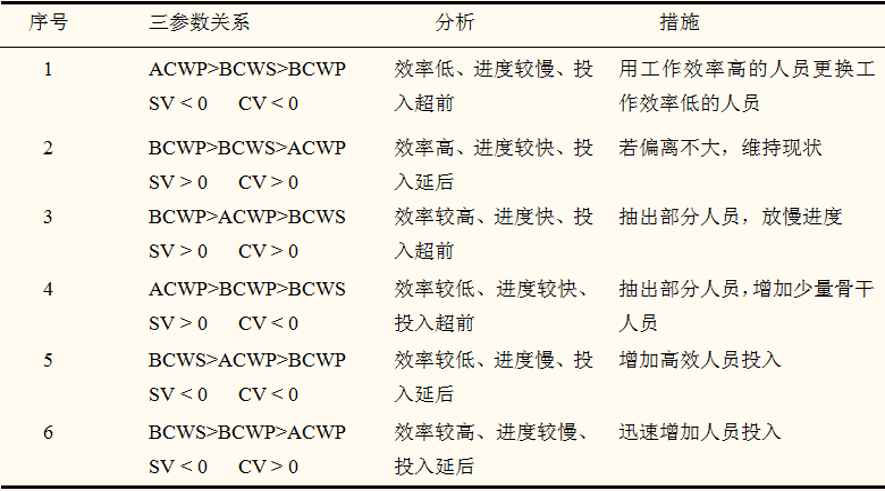
\includegraphics[width=0.8\textwidth]{image/6-3}
	\caption{挣值分析法的参数分析与应对措施}
\end{figure}
\subsection{成本控制的结果}
\begin{itemize}
	\item 修正的成本估算:为了项目的需要而修正项目的成本信息。
	\item 预算更新:对批准的成本基准所做的更新。
	\item 纠正措施:使项目将来的预期绩效与项目管理计划一致所采取的行动。
	\item 按完成情况估算:根据项目执行情况对项目总成本的预测。
	\item 项目计划的变更:当变化幅度很大时,需要产生更合适的实际成本管理计划。
	\item 经验教训:记录下产生偏差的原因、采取纠正措施的理由和其他的成本控制方面类似的经验教训。
\end{itemize}
\section{项目成本效益分析}
成本效益分析是通过比较项目的全部成本和效益来评估项目价值的一种方法。
\par 软件系统的经济效益等于因使用新软件而增加的收益加上使用新系统可以节省的运行费用。
\subsection{成本效益分析的必要性}
\begin{itemize}
	\item 效益分析将直接决定项目的可行性;
	\item 有利于项目的顺利建设,有利于组织的稳步发展;
	\item 可以帮助组织理清开支,弄清收益,从而发现问题,及时解决问题,使IT项目的运作更加有效;
	\item 有利于组织选择IT项目的投资决策,有利于组织制定IT项目的投资预算计划,有利于获得组织内部的支持。
\end{itemize}
\subsection{成本效益分析的方法}
成本效益分析方法主要有净现值法、现值指数法和内含报酬率法,这些方法的差异如图:
\begin{figure}[!h]
	\centering
	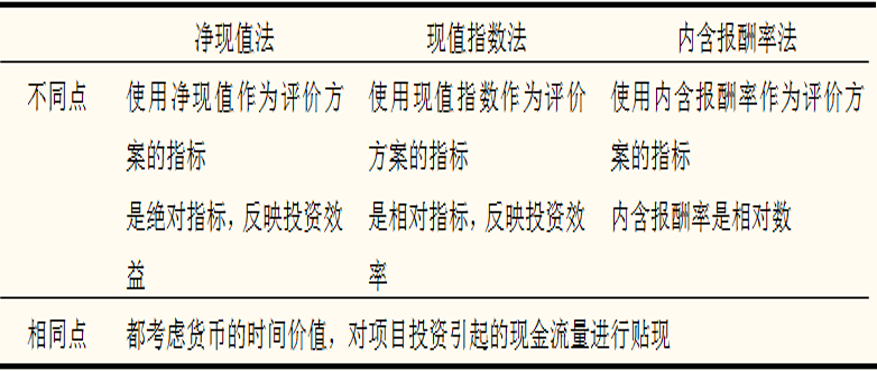
\includegraphics[width=0.8\textwidth]{image/6-4}
	\caption{净现值法、现值指数法和内含报酬率法的异同}
\end{figure}
\section{IT项目成本管理应注意的问题}
\subsection{成本估算中应该注意的问题}
成本估算仍然不精确原因:
\begin{enumerate}
	\item 软件项目是一项复杂的工作,需要巨大的努力 
	\item 没有太多的成本估算经验 
	\item 范围的不确定性和易动性 
	\item 成本估算者背景和考虑问题的角度,存在低估成本的倾向 
	\item 管理者要求做估算,但他们的重点并没有放在成本管理上
\end{enumerate}
估算成本时,要注意的问题:
\begin{enumerate}
	\item 过去的项目和现在项目之间存在的差别
	\item 软件的扩展性和维护性
	\item 开发团队对软件项目成本产生的重大影响
	\item 软件运行环境对成本的影响
\end{enumerate}
在实际项目过程中,项目成本预算存在的问题导致预算没有很好的支持项目的整体目标,甚至与之产生冲突。主要表现在:
\begin{enumerate}
	\item 对于预算在认识上存在着较大的误区
	\item 项目预算建立在对项目经理的信任的基础之上
	\item 没有全面考虑项目执行过程中可能出现的异常情况
	\item 没有充分考虑项目成本预算同项目需求之间的关系
\end{enumerate}